\section{Replacement Strategy}
\label{ch:replacement_strategy}

This chapter focuses on replacement strategy and give a brief introduction to the restricted tournament replacement (RTR). This chapter also shows the effects of RTR, the essence of distance-measure adaptation and the method of distance-measure adaptation. To reduce NFE, we use RTR to decide which individual should be replaced or be preserved. Thus, we define three types of distance measures for RTR on the permutation problems.




\subsection{Restricted Tournament Replacement}
The restricted tournament replacement (RTR) is a commonly used niching technique in the field of EDAs. RTR is also known as restricted tournament selection (RTS) which is first proposed in \citep{harik1995rts}. RTR uses the tournament strategy to decide the part which get to move on to the next generation. We present the process of RTR in algorithm \ref{alg:RTR_algorithm}, where the $Distance$ function is usually the Hamming distance in binary problems. However, Hamming distance is not suitable for the permutation problems. Thus, we define new distance for the permutation problems by characteristics of the permutation problems. In our work, the window size $w$ is suggested to set to $L/3$.


\begin{algorithm}[htbp]
    \SetKwRepeat{doWhile}{do}{while}
    \KwIn{The original population $X=\lbrace x_1, x_2, ..., x_{n-1}\rbrace$\;
    The offspring population $Y$\;
    The window size $w$\; }
    \KwOut{The population $X$ of the next generation;}
    \For{ $y\in Y$ }
    {
        Choose a random subset $S =\lbrace s_0, s_1, ..., s_{w-1}\rbrace (0\leq s_i <n)$\;
        Find the $x_{s_i}$ in $\mathop{\argmin}_{{s_i} \in S} Distance(x_{s_i},y)$\;
        \If{$Fitness(y)>Fitness(x_{s_i})$}      {
        $x_{s_i} \leftarrow y$;
        }
        
    }
    return $X$\;
    \caption{The algorithm of RTR}
    \label{alg:RTR_algorithm}
\end{algorithm}


\subsection{Distance Metric}

This subsection shows three types of distance measures for RTR on the permutation problems: edge distance, node distance and order distance. We define three distance measures by considering semantics of permutation problems.
\subsection*{Edge Distance}


An edge is connection between two nodes. The edge distance is calculated by different edge between two individuals. Let $D_{edge} (i,j)$ denote the edge distance between the two individuals $i$ and $j$, and \[ES_i=\lbrace\forall k(\pi_{(k\ mod\ L),i}, \pi_{(k+1\ mod\ L),i})\rbrace\mbox{ is an edge set of individual }i.\] Thus, $D_{edge} (i,j)$ is calculated as follows:\[D_{edge} (i,j)=L-\vert ES_i\cap ES_j\vert.\]

\begin{figure}[htbp] 
        \centering
        \begin{subfigure}{0.49\textwidth}
            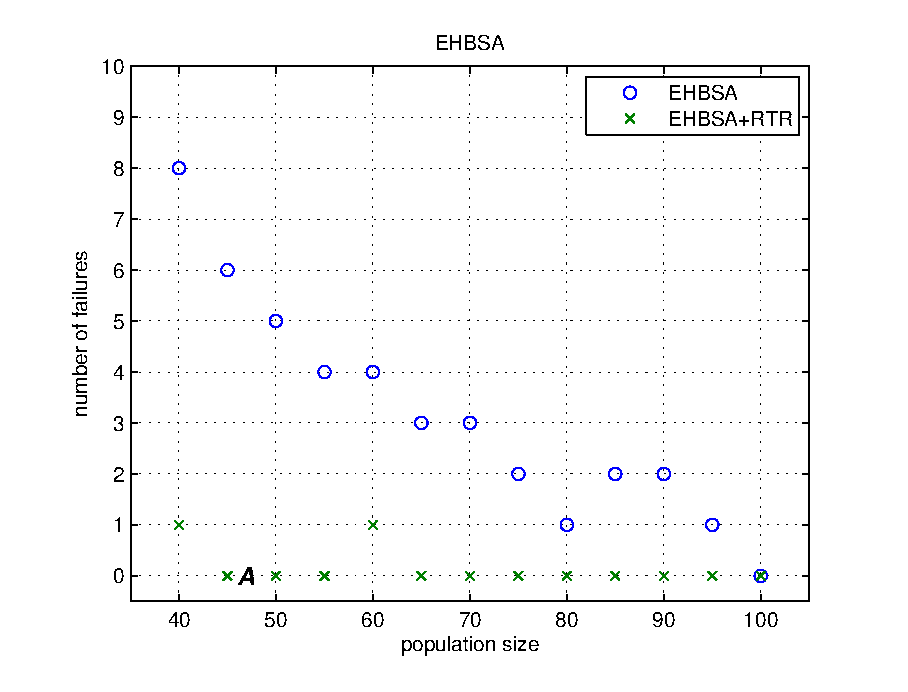
\includegraphics[width=\textwidth]{pf_a.eps}
            \caption{PopulationSize-Failures} 
        \end{subfigure}
        \begin{subfigure}{0.49\textwidth} 
            \includegraphics[width=\textwidth]{pn_a.eps}
            \caption{PopulationSize-$N_{fe}$}
        \end{subfigure}

        \caption{(Temp)Results of EHBSA on benchmark $eil51$ with template technique and $B_{ratio}=0.00$.  } 
        \label{fig:ehbsa_pf}
\end{figure}

We test EHBSA and EHBSA+RTR which uses the edge distance with different population size 20 times on benchmark $eil51$ respectively. The results are shown in Figure \ref{fig:ehbsa_pf}. The number of function evaluations increases and number of failures decreases as population size growing up. Comparing the performance of EHBSA and EHBSA+RTR, number of function evaluations of EHBSA+RTR is larger than EHBSA, but number of failures of EHBSA+RTR is the smaller than EHBSA. The point A represent the best performance of EHBSA+RTR, and it is smallest number of function evaluations among all lowest failure rate points in Figure \ref{fig:ehbsa_pf}. We get the conclusion that EHBSA+RTR with minimum required population size outperforms EHBSA. Edge distance is useful on TSP.

\subsection*{Node Distance}
The node distance is calculated by each node at different position between two individuals. Let $D_{node} (i,j)$ denote the node distance between the two individuals $i$ and $j$. $D_{node} (i,j)$ is calculated as follows:\[D_{node} (i,j)=\sum_{k=0}^{ell-1} r_{i,j} (k), \]
where $r_{i,j} (k)$ is a function defined as \[r_{i,j} (k)=
\begin{cases}
1,  & \mbox{if }\pi_{k,i}\neq \pi_{k,j} \\
0, & \mbox{otherwise}
\end{cases}
.\]


\begin{figure}[htbp] 
        \centering
        \begin{subfigure}{0.49\textwidth}
            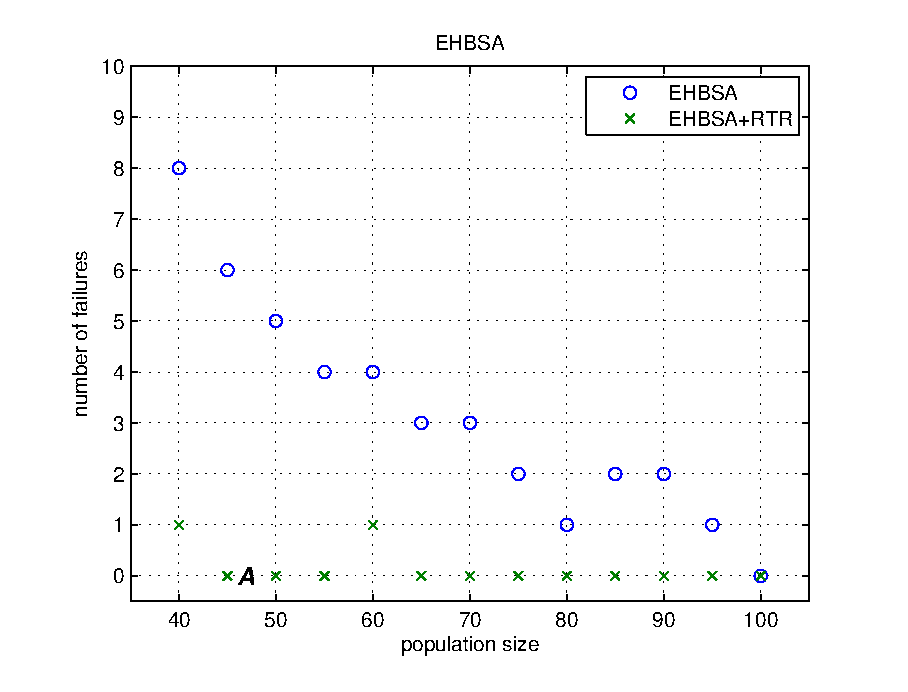
\includegraphics[width=\textwidth]{pf_a.eps}
            \caption{PopulationSize-Failures} 
        \end{subfigure}
        \begin{subfigure}{0.49\textwidth} 
            \includegraphics[width=\textwidth]{pn_a.eps}
            \caption{PopulationSize-$N_{fe}$}
        \end{subfigure}

        \caption{(Temp)Results of NHBSA on benchmark $ta031$ with template technique and $B_{ratio}=0.00$.  } 
        \label{fig:nhbsa_pf}
\end{figure}

We test NHBSA and NHBSA+RTR which uses the node distance with different population size 20 times on FSSP respectively. The results are shown in Figure \ref{fig:nhbsa_pf}. This experiment indicates that NHBSA+RTR with minimum required population size outperforms NHBSA, and node distance is useful on FSSP.



\subsection*{Order Distance}
The order distance is calculated by different orders of every node pair between two individuals. Let $D_{order} (i,j)$ denote the order distance between the two individuals $i$ and $j$. $D_{order} (i,j)$ is calculated as follows:\[D_{order} (i,j)=\sum_u \sum_v \delta_{i,j}(u,v),\]
where $\delta_{i,j} (u,v)$ is a function defined as \[\delta_{i,j} (u,v)=
\begin{cases}
0,  & \mbox{if }H_{\pi_{u}},i>H_{\pi_{v}},i\mbox{ and } }H_{\pi_{u}},j>H_{\pi_{v}},j}  \\
1, & \mbox{otherwise.}
\end{cases}
\]
In the above, $H_{\pi_{x}},i$ denotes $\pi_{x}$ of individual $i$.



\begin{figure}[htbp] 
        \centering
        \begin{subfigure}{0.49\textwidth}
            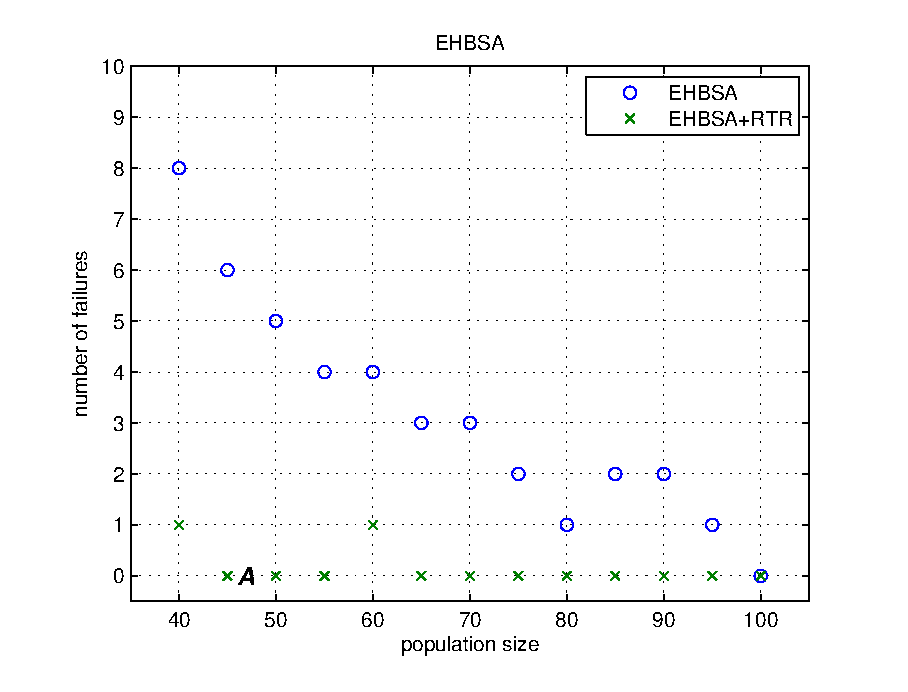
\includegraphics[width=\textwidth]{pf_a.eps}
            \caption{PopulationSize-Failures} 
        \end{subfigure}
        \begin{subfigure}{0.49\textwidth} 
            \includegraphics[width=\textwidth]{pn_a.eps}
            \caption{PopulationSize-$N_{fe}$}
        \end{subfigure}

        \caption{(Temp)Results of Enum2(EHBSA, NHBSA) on benchmark $t65i11xx$ with template technique and $B_{ratio}=0.000$.  } 
        \label{fig:order_pf}
\end{figure}


We test Enum2 and Enum2+RTR which uses the order distance with different population size 20 times on LOP respectively. The results are shown in Figure \ref{fig:nhbsa_pf}. This experiment indicates that Enum2+RTR can solve LOP more effective than Enum2, and order distance is useful on LOP.


\subsection{Essence of Distance-measure Adaptation}
This section shows the essence of distance-measure adaptation. For the same reason of essence of model adaptation(chapter \ref{ch:essence_of_adaptation}), the mechanism of distance-measure adaptation is necessary. Due to the different semantics of the permutation problems , the best fit distance measure is non-trivial.

In our experiments, we choose edge distance with the probability $p$ and choose node distance with the probability $1-p$ in each generation. The probability $p$ starts from 0.0 to 1.0 and increases 0.1 by each iteration. the instances of LOP are used : $t65b11x,t65d11x,t65f11x$ and $t65n11x$ from LOLIB. We perform independent 20 runs with the the NFE limit $E_{max} = L \times 40000$ for each iteration.
%\begin{itemize}
    %\item repeat 20 times,
    %\item test enumeration method( the EHM and the NHM are used) on LOP,
    %\item RTR is used,
    %\item the bias ratio $B_{ratio} = 0.0000$,
    %\item the NFE $E_{max} = L \times 40000$,
    %\item the edge distance and the node distance are used,
    %\item the probability $p$ starts from 0.0 to 1.0 and increases 0.1 by each iteration,
    %\item template technique is used ,
    %\item the instance of LOP : $t65b11x,t65d11x,t65f11x$ and $t65n11x$ from LOLIB ,
    %\item the cut-point number is 3 for template.
%\end{itemize}


\begin{figure}[htbp] 
        \centering
        \begin{subfigure}{0.49\textwidth}
            \includegraphics[width=\textwidth]{enum2_f.eps}
            \caption{p-Failures} 
        \end{subfigure}
        \begin{subfigure}{0.49\textwidth} 
            \includegraphics[width=\textwidth]{enum2_n.eps}
            \caption{p-$N_{fe}$}
        \end{subfigure}

        \caption{(Temp)Results of enumeration method on LOP with RTR by using the edge distance and node distance.  } 
        \label{fig:enum_pf}
\end{figure}

Figure \ref{fig:enum_pf} shows NFE and the number of failures of each probability $p$. We can find that the best performance is not at two ends of range of $p$. Therefore, best distance measure is not fixed on node distance or edge distance. This experiment indicates that mixing different distance measure can solve the permutation problems more effectively.

\subsection{Model-associated Method}
The model-associated method is a method of distance-measure adaptation. In each RTR, the model-associated method chooses the corresponding distance measure with selected model on model choosing phase. For example, let $MS=\langle m_1 , m_2, ..., m_{N_M}\rangle$ be an ordered set of models and $DS=\langle d_1 , d_2, ..., d_{N_M}\rangle$ be an ordered set of distance measures, where ${N_M}$ is the number of models. Besides, $m_i$ represents model $i$, and $d_i$ denotes the corresponding distance measure of model $i$. the model-associated method chooses the distance measure corresponding to the selected model in the model choosing phase. Table \ref{tb:model_distance} shows the models and their corresponding distance measures.


\begin{table}[htbp]
    \centering
    \begin{tabular}{|l|l|}
    \hline
    \textbf{Semantic Models}       & \textbf{Corresponding Distance}  \\ \hline
    \textbf{NHM} & node     	 \\ \hline
    \textbf{EHM} & edge   	\\ \hline
    \textbf{the PL model} & order   	\\ \hline
  
    \end{tabular} 
    \caption{Corresponding distance measures of models}
    \label{tb:model_distance}
\end{table}

To investigate the performance of the model-associated method, we test Enum2+RTR by using the edge distance, the node distance and the model-associated method on LOP with the NFE limit $E_{max} = L \times 40000$. %The experiment settings are as follows:
%\begin{itemize}
    %\item repeat 20 times,
    %\item test enumeration method( the EHM and the NHM are used) on LOP,
    %\item RTR is used,
    %\item the bias ratio $B_{ratio} = 0.0000$,
    %\item the NFE $E_{max} = L \times 40000$,
    %\item the edge distance , the node distance and the model-associated method are used,
    %\item template technique is used ,
    %\item the instance of LOP : $t65b11x,t65d11x,t65f11x$ and $t65n11x$ from LOLIB ,
    %\item the cut-point number is 3 for template.
%\end{itemize}
\subsection{Reward Policy}
\subsection{Window Size}
\subsection{Empirical Study}
This section shows the performance of MABMA+RTR on the different permutation problems. For comparison, MABMA-UCB, MABMA-UCBT, MABMA-UCB+RTR, MABMA-UCBT+RTR are tested on LOP,TSP,QAP and VRPTW. In the experiment of the model-associated method, EHM, NHM and the PL model are used. For each instance, we perform independent 20 runs with the NFE limit $E_{max} = L \times 40000$.
%\begin{itemize}
    %\item repeat 20 times,
    %\item test MABMA(EHBSA, NHBSA and PLEDA are used) on LOP,TSP,FSSP and CVRP,
    %\item RTR is used,
    %\item the bias ratio $B_{ratio} = 0.0000$,
    %\item the NFE $E_{max} = L \times 40000$,
    %\item the model-associated method is used,
    %\item template technique is used ,
    %\item the cut-point number is 3 for template.
%\end{itemize}


